% DOCUMENT FORMATING
\documentclass[12pt]{article}
\usepackage[margin=1in]{geometry}

% PACKAGES
\usepackage{amsmath} % For extended formatting
\usepackage{amssymb} % For math symbols
\usepackage{amsthm} % For proof environment
\usepackage{array} % For tables
\usepackage{enumerate} % For lists
\usepackage{extramarks} % For headers and footers
\usepackage{fancyhdr} % For custom headers
\usepackage{graphicx} % For inserting images
\usepackage{multicol} % For multiple columns
\usepackage{verbatim} % For displaying code
\usepackage{tkz-euclide}
\usepackage{pgfplots}
\usepackage{mathtools}


% SET UP HEADER AND FOOTER
\pagestyle{fancy}
\lhead{\MyCourse} % Top left header
%\chead{\MyTopicTitle} % Top center header
\rhead{\MyAssignment} % Top right header
%\lfoot{\MyCampus} % Bottom left footer
\cfoot{} % Bottom center footer
%\rfoot{\MySemester} % Bottom right footer
\renewcommand\headrulewidth{0.4pt} % Size of the header rule
\renewcommand\footrulewidth{0.4pt} % Size of the footer rule




% ----------
% TITLES AND NAMES 
% ----------

\newcommand{\MyCourse}{Math 241}
\newcommand{\MyAssignment}{Worksheet 8}
%\newcommand{\MySemester}{Spring 2020}
%\newcommand{\MyCampus}{University of Hawaii at Manoa}

% ----------
% BEGIN DOCUMENT
% ----------
\begin{document}
\begin{enumerate}

\item Find the following limits at infinity if they exist. If it is $\infty$ or $-\infty$, state which.

\begin{enumerate}
\item $\displaystyle\lim_{x\to\infty} \dfrac{6(3x^2-1)^3}{x^2(2+3x^2)(3-2x)^2}$
    \vspace{3in}

    \item $\displaystyle\lim_{x\to\infty} (x-\sqrt{x})$
    \vfill
\end{enumerate}

\pagebreak

\pgfplotsset%Default tikz axis style
{
    width=10cm, height=5cm,
    axis lines=center, 
    grid,
    grid style={very thin, dotted, black!50},
    xmin=-5,    xmax=5,         xtick distance=1,
    ymin=-5,    ymax=5,         ytick distance=1,
    restrict y to domain=-10:10, % <-------
    ticklabel style={font=\scriptsize, fill=white, inner sep=2pt},
    domain=-5:5, samples=100,
    no marks, 
    every axis plot post/.append style={ultra thick, semitransparent,},
}

\item Consider the function $f(x) = \dfrac{x^2-4}{x^2+1}$ with the following properties. \textbf{(You do not need to check these properties. In particular, you do not need to differentiate this function).}
\begin{itemize}
    \item $f$ has $x$-intercepts at $x=\pm 2$ and a $y$-intercept at $y=-4$.
    \item $f$ has a horizontal asymptote $y=1$ and no vertical asymptotes.
    \item $f, f',$ and $f''$ are defined for all values of $x$.
    \item $f'(x)$ is negative on $(-\infty,0)$ and positive on $(0,\infty)$.
    \item $f''(x)$ is negative on the open intervals $\left(-\infty,-\frac{1}{\sqrt{3}}\right)$ and $\left(\frac{1}{\sqrt{3}},\infty\right)$. Note that $\frac{1}{\sqrt{3}}\approx .6$
    \item $f''(x)$ is positive on the open interval $\left( -\frac{1}{\sqrt{3}},\frac{1}{\sqrt{3}}\right).$
\end{itemize}
\begin{enumerate}
    \item Does $f$ have any local extrema? If so, state what type they are and the $x$-value where they occur.
    \vfill
    \item Does the graph of $f$ have any inflection points? If so, give the $x$-coordinate(s).
    \vfill    
    \item Using the information above, sketch the graph of $f$ on the axes below. Clearly mark the horizontal asymptote, $x$ and $y$ intercepts and any inflection points.
    \begin{center}
            \begin{tikzpicture}
                \begin{axis}
                [
                    scale=1.5,
                    xmin=-8.1, xmax=8.1,
                    ymin=-5.1, ymax=2.1,
                    xtick distance=1,
                    ytick distance=1,
                    declare function={f(\x)=\x*\x;}
                ]
                \end{axis}
            \end{tikzpicture}
        \end{center}
%    \begin{center}
%        \includegraphics[width=0.65\textwidth]{Images/Blankgraph.jpeg}
%    \end{center}
\end{enumerate}
\pagebreak

\item A farmer has 600 ft of fencing to enclose a rectangular field which he plans to subdivide into two pens of equal area, see image below. He plans to use the bank of a straight river as one side of the fence, so he does not need fencing along the river. What is the largest possible area of the field? \emph{Hint:} $600=3x+y$.
    \begin{center}
    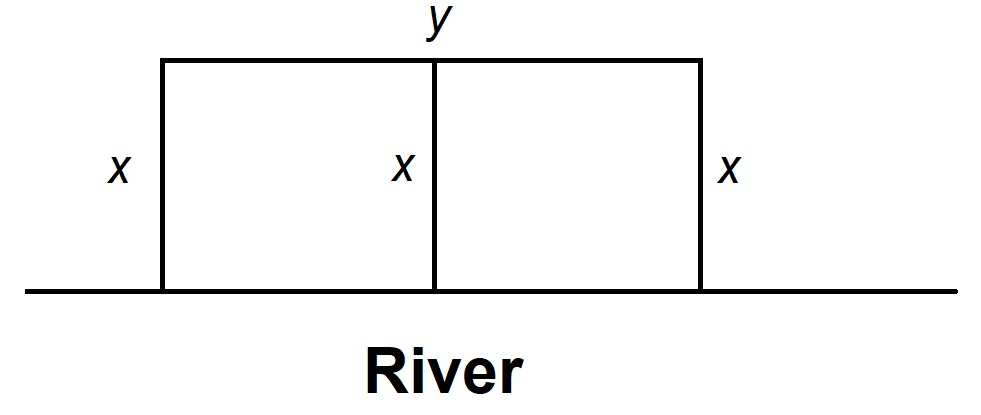
\includegraphics[scale=0.25]{Images/S23M241MT3pic1.jpg}
    \end{center}

\pagebreak

\item Find the point on the curve $y=\sqrt{x}$ that is closest to the point $(3,0).$
\end{enumerate}
\end{document}